\section{Analysis}
\label{s:DataGAAnalysis}

By generating a certain amount of packets, captures makes a valid number for conducting a comparative analysis on the synthetic generated data sets.
During this research, the main analysis component chosen was the Jupyter notebook.

%% ---------------------------- JUPYTER NOTEBOOK ----------------------------
\subsection{Jupyter notebook}
\label{s:AnalysisJupyter}
Jupyter notebook is a non-cost web application used for editing code in the browser, which includes tab completion, highlighting, and indentation. Jupyter has the ability to display media formats such as LaTeX, images, and HTML. It also supports markdown language for adding text in an easily readable format which in the browser is compiled into HTML for the user. This enhances the readability for further commenting code by using for mating and is not only limited to code comments.
The documents for Jupyter is called notebooks, which are JSON file containing computational session data recorded during a session \autocite{electronics10151849, jupyter}.
This means that when data are inserted, such as in this packet capture research, it is recorded in the \textit{.ipynb} file. When conducting packet capture analysis and reading amounts of data into the notebook, the processed data are stored, which streamlines the process of analysis of the data.
The structure of a notebook is divided into cells, where either code, text, or media can be inserted and executed.
Other useful features include popular used export formats such as LaTeX compiled PDF, Python, LaTeX, and HTML.
A notebook can be easily opened when shared only by having Jupyter installed and running, without the need of re-running the notebook since all data already are saved as a checkpoint.
Jupyter has the capability of running all code in one single push, which enables a semi-automatic analysis with the base in a notebook template.

Jupyter uses the underlying Python on the Jupyter host machine, which enables the use of all installed libraries on the machine.
A capture of a part of the Jupyter notebook is shown in figure \ref{fig:JupyterScreenshot}.
The figure shows a code snippet that generates a plot of packet number correlated with destination ports and colorized with source ports, which represents scan number.
At the top of the figure, a play button is shown, which enables the user of the notebook to execute the code within the notebook, and the results are represented either in a plot, raw text format, or table format.
Another important feature in the Jupyter notebook is the checkpoint feature, which enables users to save the notebook in a given state for later use. This enables the possibility of sharing the notebook in the current state containing the data at a given stage for other users to review the results.

\begin{figure}[!htbp]
\centerline{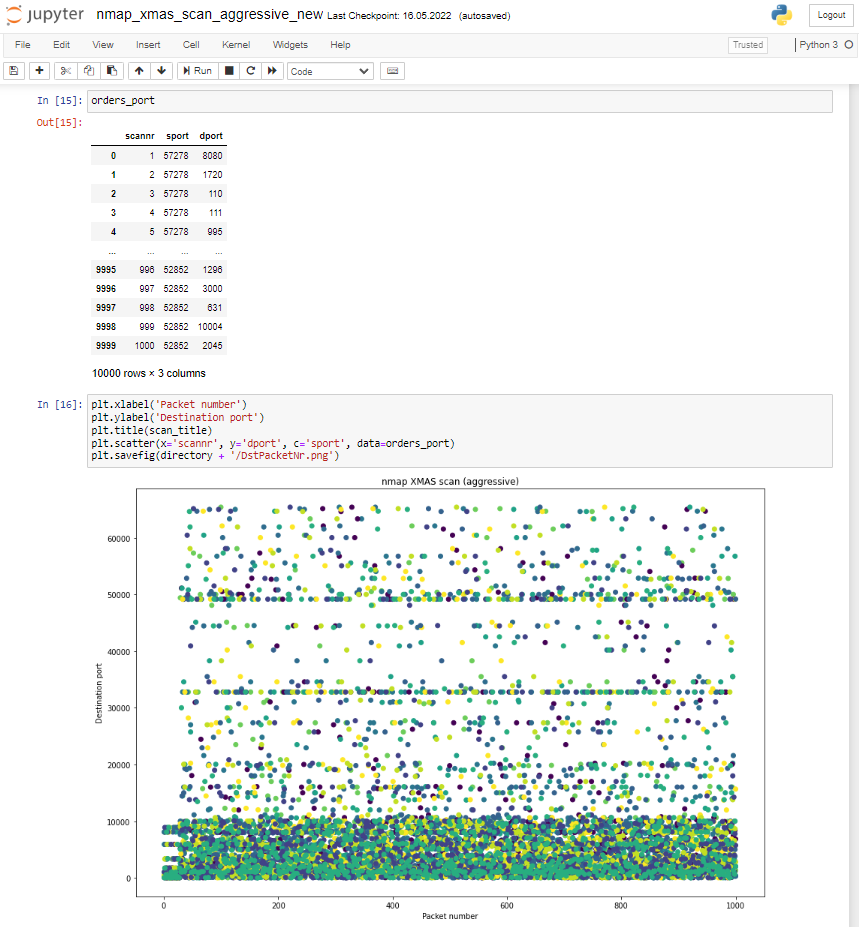
\includegraphics[scale=0.55]{images/analysis/JupyterScreenshot.PNG}}
\caption{Capture of a part of the Jupyter notebook.}
\label{fig:JupyterScreenshot}
\end{figure}
%% ---------------------------- /JUPYTER NOTEBOOK ----------------------------


%% ---------------------------- PYTHON LIBRARIES FOR ANALYSIS ----------------------------
\subsection{Python libraries for analysis}
\label{s:AnalysisPythonLibrary}

A popular Python library called \textsc{matplotlib} is often used for visualization, and this is supported in Jupyter.
The visualizations in this research use matplotlib for plotting data for visualization, as shown in figure \ref{fig:JupyterScreenshot}.
The Pandas library\footnote{https://pandas.pydata.org/} is a Python-built analysis tool that is used in this analysis.
In listing \ref{lst:JupyterPandaImportCSV} the data from given CSV files in a directory are imported into a Panda DataFrame in line 9. This is later used as an important data format for the whole analysis.


\begin{table}[!htbp]
\caption{Python libraries used in analysis}
\begin{center}
\begin{tabular}{|l|l|}
\hline
\textbf{Library} & \textbf{Usage}\\
\hline
matplotlib.pyplot & Used for plot generation.\\
\hline
matplotlib.cm & Used for rainbow color generation.\\
\hline
pandas & Used for reading CSV files into Panda DataFrames for later use in data\\
& visualisation in plots with matplotlib.plot and table forms.\\
\hline
numpy & Used for numeric sequence creation for use in matplotlib to generate rainbow\\
& colors in plots.\\
\hline
os & Used for reading directory contents, checking file existence and and extracting\\
& file names.\\
\hline
\end{tabular}
\label{tbl:PythonLibsAnalysis}
\end{center}
\end{table}


\begin{listing}[!ht]
\caption{Importing data from CSV files and generate Panda dataset in Jupyter}
\label{lst:JupyterPandaImportCSV}
\begin{minted}[linenos]{Python}
directory = '/home/user/notebooks/pcaps/nmap_xmas_scan_aggressive'
scan_list = []

for filename in os.listdir(directory):
    f = os.path.join(directory, filename)
    if os.path.isfile(f):
        filename, ext = os.path.splitext(f)
        if ext == '.csv':
            read = pd.read_csv(f)
            if read.empty:
                pass
            else:
                scan_list.append(read)
\end{minted}
\end{listing}


%% ---------------------------- ABOUT THE ANALYSIS ----------------------------
\subsection{Analysis methodology}
\label{s:AnalysisMethod}
%\ref{s:AnalysisMethod}
The analysis in Jupyter in this research is built up as a Jupyter template.
This template is reused for the various types of scans and also for the various timing templates.

The notebook is structured with an import section where the chosen libraries are imported, the IP address to the scanning host is defined, and the title of the scan is defined.
The IP address to the scanning host is defined for later in the process to filter out only incoming packets and not outgoing packets to the scanning host.
Further the CSV files processed with the \textsc{packet capture parser}, described in section \ref{ss:PcapParser}, are imported to a Panda data frame.

The analysis then goes into investigating the duration of each scan for the chosen timing template and scan type.
A histogram is generated and visualizes the count of scans related to the duration of the scan.
Figure \ref{fig:PingSvcInsAgrNormHist} shows the histogram for various scanning types and timing templates, which is the first analysis visualization for each of the given scans in this research's Jupyter notebook.
Measurements for establishing the minimal and maximum time used, the standard deviation, and the average are also visualized in a table, such as a table \ref{tbl:StandOutScanDuration}.

During the next two sections in the notebook, the packet count and packets per second are measured in order to identify any eventual anomalies in sent and received packets.
Comparing the average packets per second rate to the used timing template can give an indicator of how fast or slow the scan is conducted.

Further, the orders of ports scanned are logged in order to spot similarities for which ports are scanned in which order.
The similarities could easily be seen in a figure where each scan is represented in its own color, such as in figure \ref{fig:DstPortSequenceMisc}.
Other statistical measurements were also conducted during this research, among visualizing source ports to destination ports on one single scan by visualizing the scan number and destination ports in a diagram results in a good visualization of locating where the main number of ports have been scanned. This would be described in the results in section \ref{s:DestinationPortPatterns}.
The importance of visualizing the scans gains a higher situational awareness of what is going on in each scan, and it simplifies the analysis of spotting anomalies and patterns.

A mathematical code computation was created to figure out each of the packet sizes for each received packet from the scanning host. The main reason behind this was to establish an eventual deviation from the "standard" packet size for each received packet. This will be further elaborated in the results chapter under section \ref{s:DesignImplementSummary}.

Other analysis parameters added to the analysis are the TCP window size and sequence number.
Extraction of the TCP window size was added to easily spot abnormal window sizes.
The sequence number is used for comparison against which number of scans is conducted, destination port, and source ports.
These measurements are not further described within this research, but further analysis information is located within the Jupyter notebooks for the respective scans.
